% !Mode:: "TeX:UTF-8"
\chapter{问题分析}
\section{车牌规格}

我国目前使用的汽车牌号标准是 2007 开开始实施的《中华人民共和国机动车号牌》GA36­2007(2010 开修订)。根据
GA36­2007 对机动车牌号编排规则规定,我国汽车的车牌构造特点如下:

\begin{enumerate}
\item汽车车牌号的编排规则:我国的标准车辆车牌是由一个省份汉字(军警车牌为其他汉字)后跟字母或阿拉伯数字组成
的 7 个字序列。
\item标准车牌的的具体排列格式是:X1X2∙X3X4X5X6X7,X1是各省、直辖市的简称或军警,X2是英文字
母,代表该汽车所在地的地市代码,比如 A 代表省会,B 代表该省的第二大城市,C 代表该省的第三大城市,
X3X4X5X6X7为英文字母或阿拉伯数字,2010开以前车牌号码的分布规律是,前面是字母,后面是数字。
\item 但是,随着车
辆保有量的增加,每个字母所属号段越来越不够用。按照新《中华人民共和国机动车号牌》(2010 开修订)标准,将允
许字母在后五位编码中任意一位出现,但不能超过两个。除了第一个汉字外,字母和数字的笔画在竖直方向都是联通的。
\end{enumerate}

\begin{figure}[h]
	\centering
	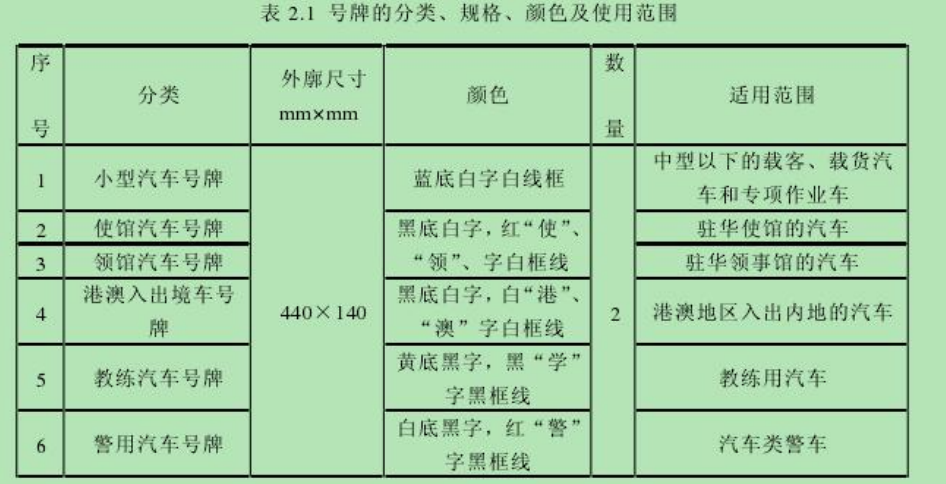
\includegraphics[scale=0.5]{figures/3.png}
	\caption{牌照类型图}
	\label{fig:1}
\end{figure}

绝大部分的汽车牌照的宽度为1100px,高度为350px,牌照上一共有7个或8个字符,其中,每个字符的宽度为45mm,高
度为90mm,间隔符的宽度为10mm,除了第二个和第三个字符之间的间距为 34mm 外,字符之间的间隔宽度12mm。民
用的汽车牌照上有所属省、自治区或直辖市的简称(军用、警察牌为其他汉字),监督机关及发证照的代号(大写的英文字
母)后跟阿拉伯数字或英文字母组成的7个字符序列。

\begin{figure}[h]
	\centering
	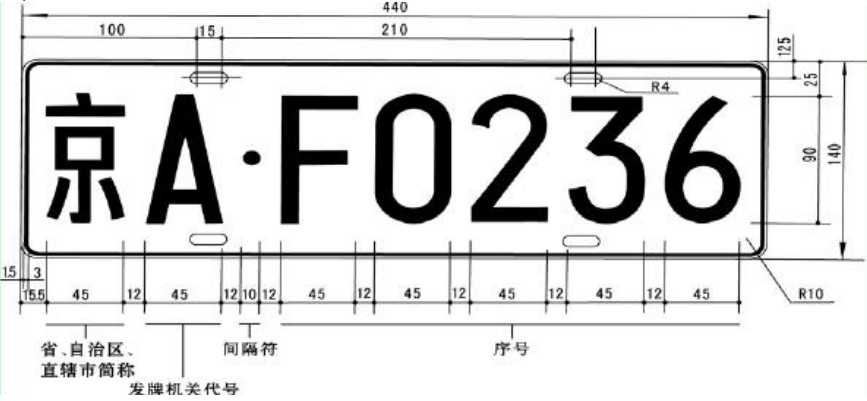
\includegraphics[scale=0.5]{figures/4.png}
	\caption{牌照设计图}
	\label{fig:1}
\end{figure}


\section{归纳特征}
\begin{enumerate}
	\item 有两种或这三种颜色组成
	\item车牌具有统一的标准尺寸 宽:高=3.14,这便于字符的分割和车牌的定位。字符的面积大约占整个车牌面积的
	20%
	\item边缘特征:汽车的车牌边框是有规则的边缘,由于汽车车牌的字符排列规则,汽车车牌的垂直边缘比水平边缘更
	为丰富,而汽车的车身却有丰富的水平边缘,垂直边缘不明显。
	\item黑白跳变特征:车牌区域二值化后,字符和背景为一黑一白,存在明显的黑白跳变,且跳变的次数在一定范围
	内。
	\item投影特征:汽车车牌图像进行垂直投影后的图像是由波峰、波谷交替组成的连续分布图,垂直投影后的图像会有
	约七个波峰或波谷区;汽车车牌图像进行水平投影后的图像中灰度跳变的像素点数累加值很大。
\end{enumerate}
\begin{figure}[h]
	\centering
	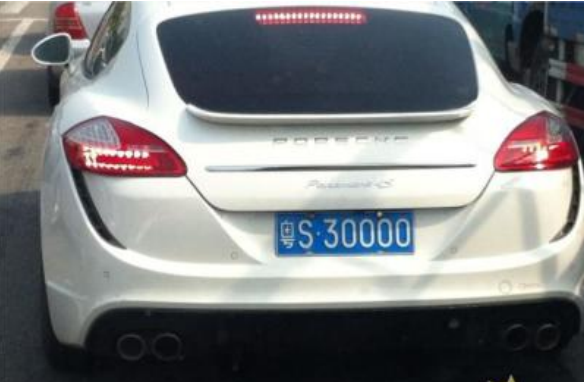
\includegraphics[scale=0.5]{figures/1.png}
	\caption{相机抓拍的车辆图片}
	\label{fig:1}
\end{figure}

了解我国车牌的特征,有利于后续对车牌进行的各种操作,在项目步骤中,这属于对需求目标的全面了解。对
车牌的了解不能跳过,因清楚的知道我们所要处理的的目标的各个特性,这样才有利于我们利用这些特性来操作车
票图像。
